\documentclass[12pt,a4paper]{article}
\usepackage{fontspec, xunicode, xltxtra}
\XeTeXlinebreaklocale "zh"
\XeTeXlinebreakskip = 0.1pt plus 1pt minus 0.1pt
\usepackage{xeCJK} 
\usepackage{fontspec}  
\setCJKmainfont{SimSun} 
\setCJKmonofont{SimSun} 
\setmainfont{Courier}%{Times New Roman} {SourceCodePro-Regular}{Consolas}{Courier}
\usepackage{indentfirst} 
\setlength{\parindent}{2em}
\usepackage{float}
\usepackage[utf8]{inputenc}
\usepackage{setspace}
\usepackage[colorlinks,linkcolor=black,anchorcolor=black,citecolor=black]{hyperref}
\usepackage{amsmath}
\usepackage{amsfonts}
\usepackage{amssymb}
\usepackage{geometry}
\geometry{left=2.5cm,right=2.5cm,top=2.5cm,bottom=4cm}
\usepackage{listings}
\lstset{language=C++}
\lstset{breaklines}
\lstset{extendedchars=false}
\usepackage{fancyhdr}
\pagestyle{fancy}
\lhead{数据结构大作业报告}
\author{姚皓天(2013011515)}
\title{数据结构大作业报告\\红黑树}
\date{2014年12月}
\graphicspath{{Figure/}}
\begin{document}
\maketitle
\thispagestyle{empty}

\newpage
\thispagestyle{empty}
\renewcommand\contentsname{\textbf{目录}}
\tableofcontents

\newpage
\section{基本原理}
\subsection{概述}
本程序是由 Microsoft Visual Studio 2012 创建,目标框架为 .NET Framework 4.5。
程序实现了红黑树数据结构的可视化,实现了对学生成绩信息的输入输出以及检索的功能。
此外,实现了Hash表,用于管理学生的姓名和学号数据。
\subsection{原理}
首先实现了将学生封装为Student类,接着封装为Node类,并在基础上创建红黑树,RBTree类。接着创建了HashTable<T>模板,实现了Hash表的功能。最后,在.NET框架下,完成图形界面的部署。
\subsection{界面}
\begin{figure}[H]
\centering
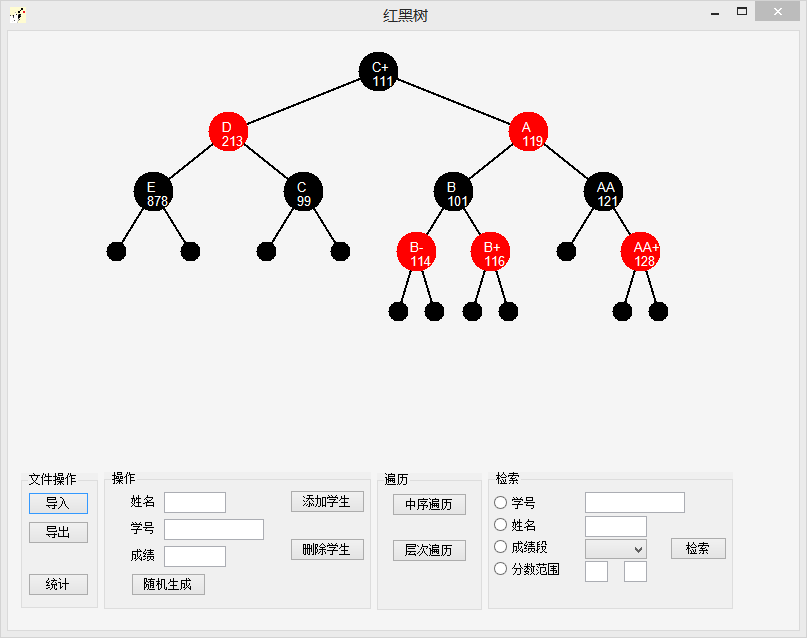
\includegraphics[width=0.8\textwidth]{2.png}
\caption{界面} 
\end{figure}
\subsection{操作说明}
\subsubsection{文件操作}
导入,导出按钮,可以从文本文件导入数据,或者导出到文本文件。统计信息按键可以显示实时的统计信息。
\subsubsection{添加删除}
输入学生的信息,就可以添加学生的信息,同时,上方的界面将同步绘制响应的红黑树可视化界面。输入学生的学号,就可以删除对应的学生。
\subsubsection{红黑树可视化}
点击节点,可以在弹出的对话框中查看节点的信息,同时在对话框中选中的条目信息可以回填到主界面中。
\subsubsection{遍历}
可以实现中序遍历和层次遍历两种方式的遍历。
\subsubsection{检索}
可以选择通过,姓名,学号,成绩段和分数区间四种不同的方式来检索学生成绩信息。
\section{程序设计}
\subsection{需求分析}
程序需要实现红黑树及其可视化,以及Hash表的功能。
\subsection{概要设计}
首先实现了将学生封装为Student类,接着封装为Node类,并在基础上创建红黑树,RBTree类。接着创建了HashTable<T>模板,实现了Hash表的功能。最后,在.NET框架下,完成图形界面的部署。
\begin{figure}[H]
\centering
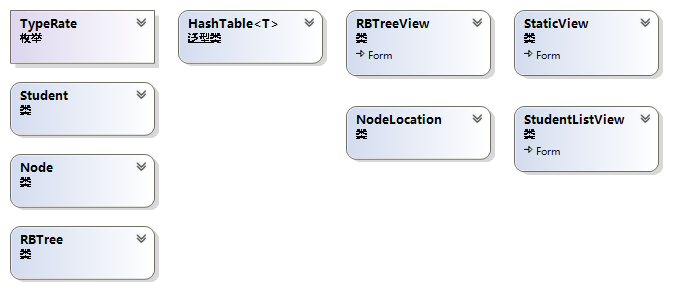
\includegraphics[width=0.8\textwidth]{1.png}
\caption{类图} 
\end{figure}
\subsection{详细设计}
\subsubsection{Student类}
\begin{figure}[H]
\centering
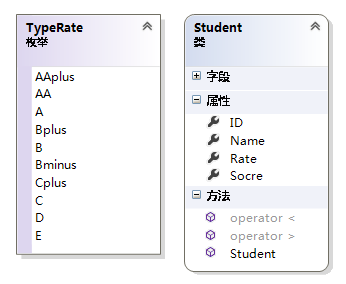
\includegraphics[scale = 1]{3.png}
\caption{Student类} 
\end{figure}
枚举型TypeRate描述成绩段。\par
Student类封装了学生的属性,并重载了operator< 和 opeartor > 通过分数段来实现对学生的比较,便于在红黑树中进行操作。
\subsubsection{RBTree类}
\begin{figure}[H]
\centering
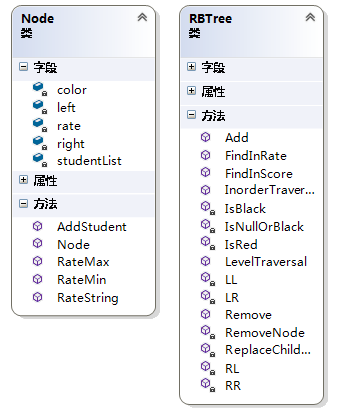
\includegraphics[scale = 1]{4.png}
\caption{红黑树的实现} 
\end{figure}
Node为红黑树中的每一个节点,包含的字段有颜色,关键码,左右子树,以及一个线性表用于保存数据。\par
RBTree实现了红黑树的插入,删除,查找,遍历等方法。其中树的旋转,换底作为私有方法,用于红黑树的维护。
\subsubsection{HashTable类}
\begin{figure}[H]
\centering
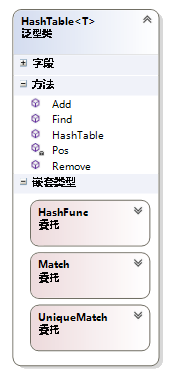
\includegraphics[scale = 1]{5.png}
\caption{HashTable的实现} 
\end{figure}
HashTable用泛型编写,实现添加,删除以及查找的功能。Hash函数的实现,查找匹配的方法使用委托编写,在实例化时实现。
\section{设计心得}
\subsection{收获}
这次大作业抛弃了年代久远的MFC框架,在全新的.NET Framework 4.5框架下完成了此处程序的编写。主要收获是熟悉了.NET Framework 以及编程语言C$\sharp$。
\subsection{特色}
程序界面简洁。
\section{文件清单}
\begin{itemize}
\item src$\backslash$ 工程文件
\begin{itemize}
\item Student.cs Student类,对学生各种属性进行封装
\item RBTree.cs RBTree类,实现红黑树
\item HashTable.cs HashTable<T>模板,实现哈希表功能
\item RBTreeView.cs 程序主界面
\item StudentListView.cs 列出学生信息的对话框
\item StaticView.cs 统计信息对话框
\end{itemize}
\item bin$\backslash$ 可执行文件
\item doc$\backslash$ 文档
\end{itemize}
程序版本库:\url{https://github.com/yht1995/RBTree.git}
\end{document}